\chapter{Konzept}

\begin{figure}[b]
	\centering
	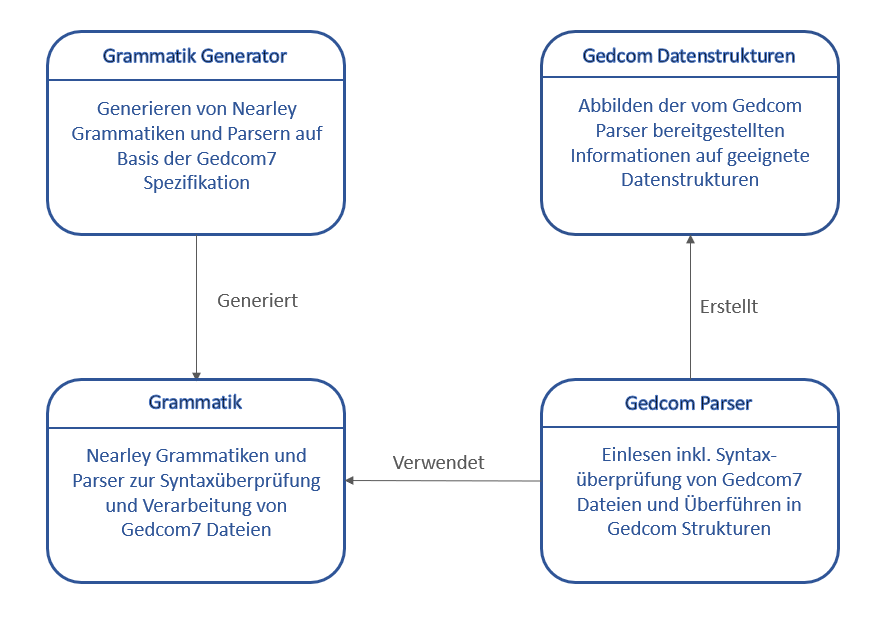
\includegraphics[width=0.8\textwidth]{images/konzept_allgemein.png}
	\caption{Allgemeiner Aufbau}
	\label{fig: Allgemeiner Aufbau}
\end{figure}

\label{chap: Konzept}
Die Bibliothek \textit{gedcom7.js} lässt sich wie in \hyperref[fig: Allgemeiner Aufbau]{Abbildung 4.1} dargestellt in vier logische Teile gliedern. Das zentrale Element ist der \textsc{Gedcom Parser}, mit dem Dateien oder Strings im Format Gedcom7 eingelesen werden und mit Hilfe von \hyperref[sec: Nearley]{\textit{Nearley}} auf Korrektheit der Syntax überprüft werden können. Die dafür zugrundeliegende Grammatik wird mit Hilfe eines \textit{Grammar Generators} generiert, der die in \cite{GEDCOM} definierte Spezifikation in eine nearley-konforme Syntax überführt. Die so eingelesenen Informationen werden in Gedcom Strukturen gespeichert, die verändert und erweitert werden und anschließend im Format Gedcom7 ausgegeben werden können. In den folgenden Abschnitten werden die vier Teile und das Zusammenspiel dieser in detaillierter Form vorgestellt.

\section{Grammatik Generator}
\label{Grammatik Generator}
asdasd

\section{Gedcom Grammatik}
\label{Gedcom Grammatik}
asdasd

\section{Gedcom Struktur \& Parser}
\label{Gedcom Struktur und Parser}
asdasd

